\documentclass[a4paper]{article}
\usepackage[utf8]{inputenc}
\usepackage[T1]{fontenc}
\usepackage[bookmarks,colorlinks]{hyperref}
\usepackage[french]{babel}
\usepackage{pdfpages}

\title{Rapport d'analyse du projet de Technologies Objets}
\author{Maxime Arthaud \and Korantin Auguste \and Martin Carton}
\date{24 Mai 2013}

\begin{document}
\maketitle

\section{Scénarios d'utilisation}
  Génération d'image à partir d'une scène 3d comportant des objets simples.

\section{Diagramme d'analyse}
  \begin{centering}
    \centerline{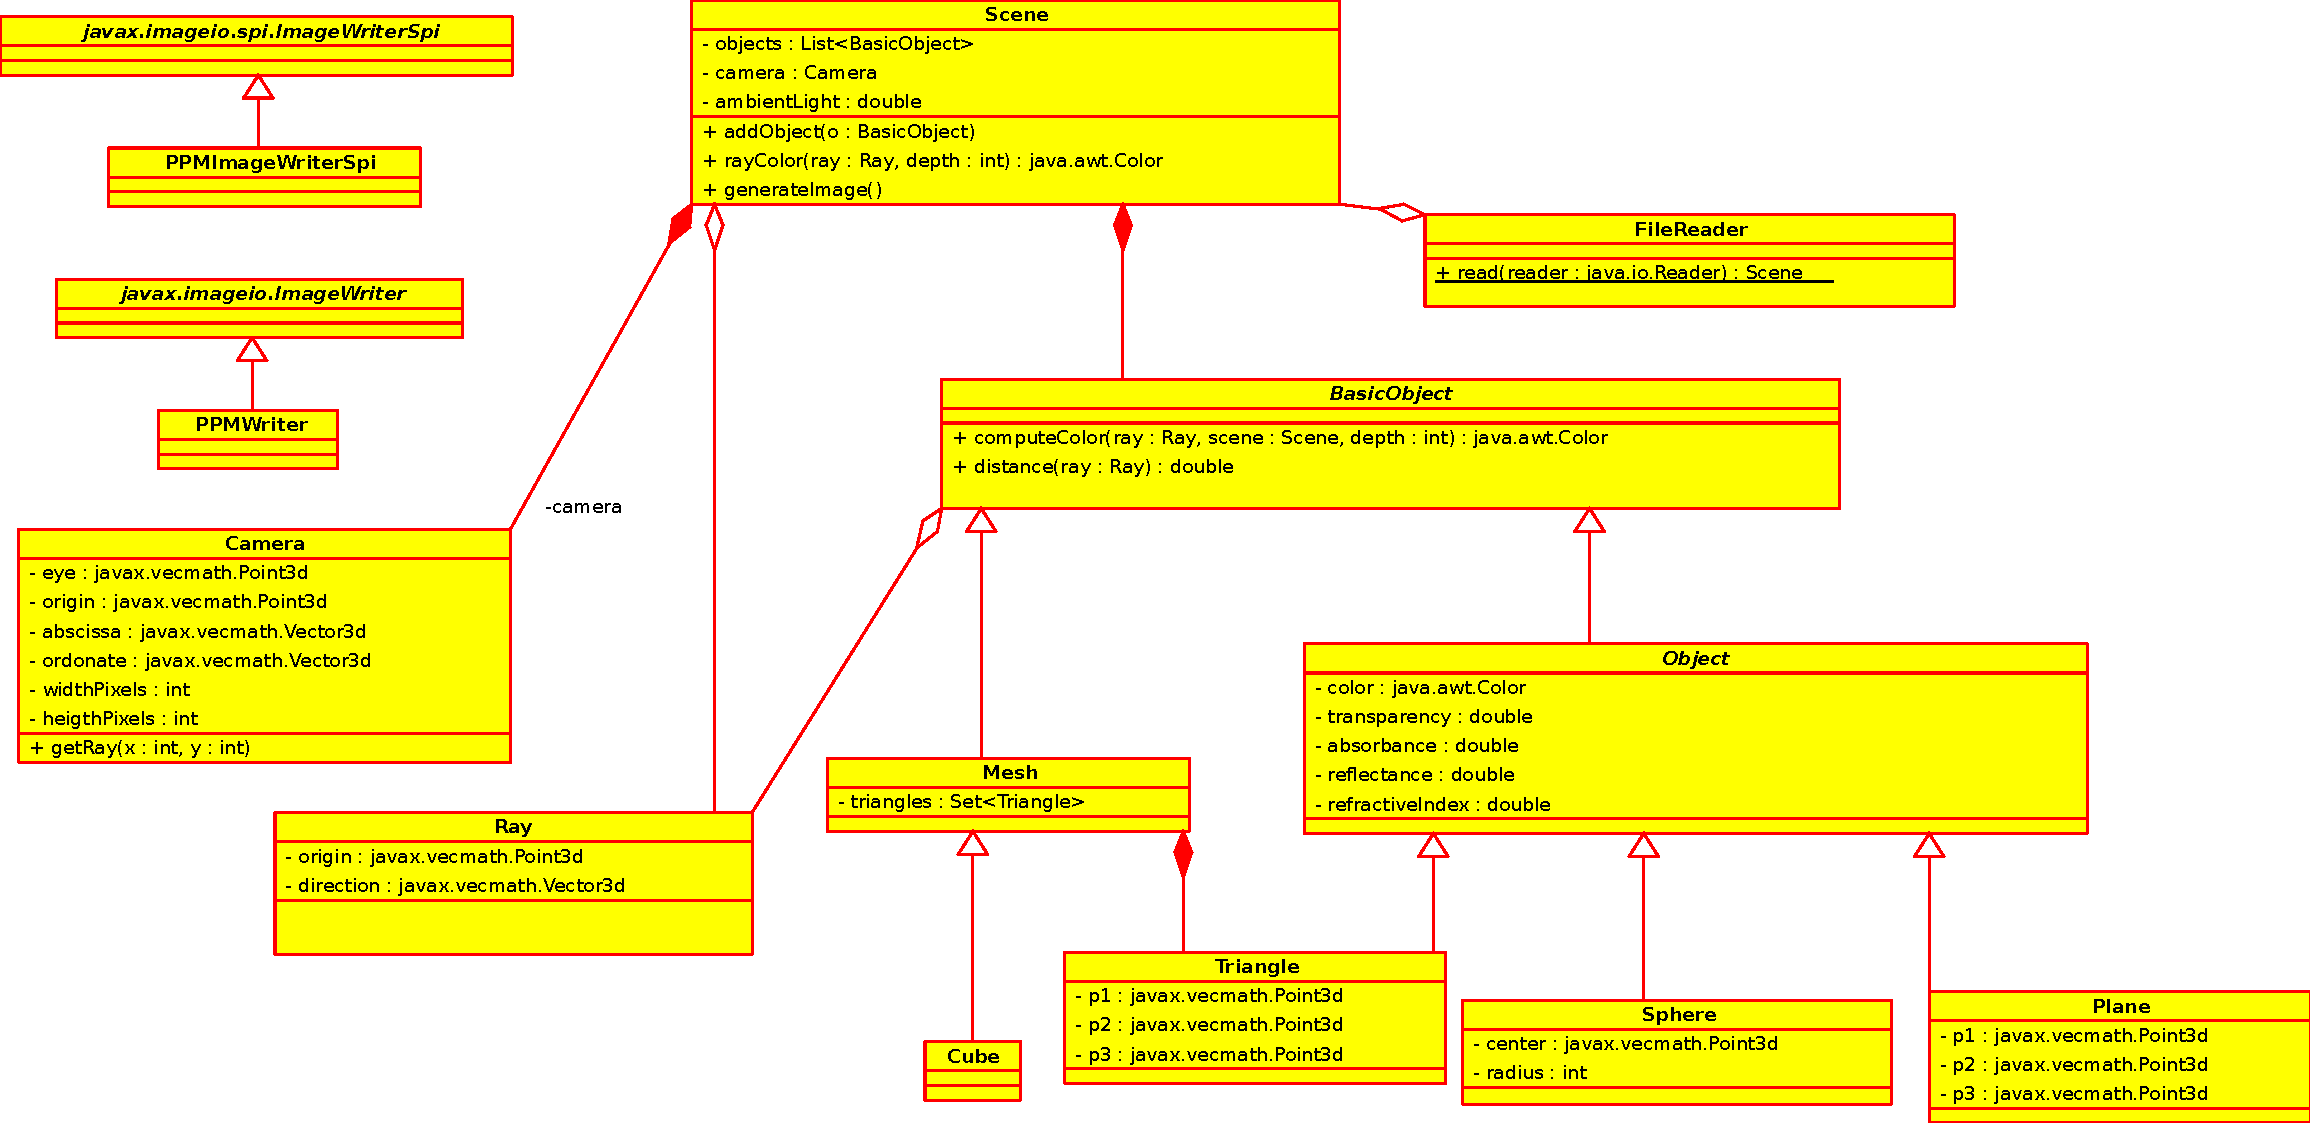
\includegraphics[width=1.5\textwidth]{uml.pdf}}
  \end{centering}
  Présenter un peu toutes les classes.

%\section{Diagramme de séquence}
\section{Interface utilisateur}
  \begin{centering}
    \centerline{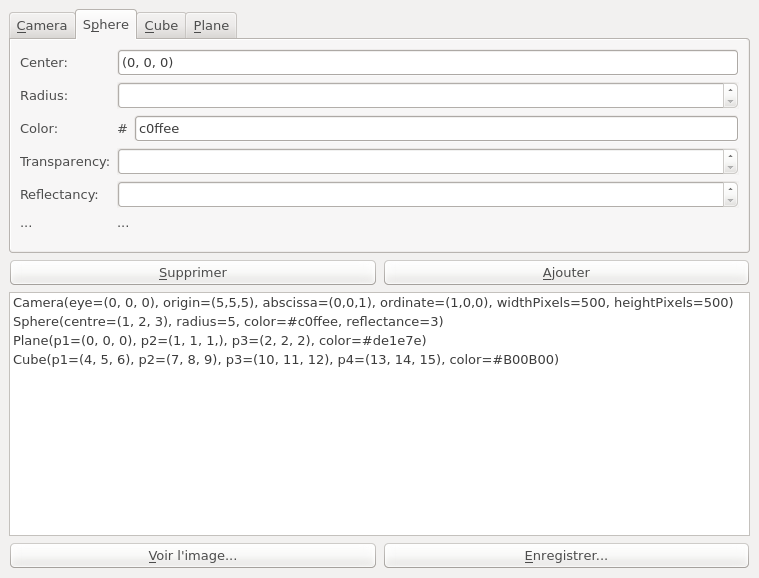
\includegraphics[width=1.5\textwidth]{gui.png}}
  \end{centering}
\section{Démarche}
\section{Tâches effectuées}
\end{document}

